\documentclass[mingoth,11pt,a4j,uplatex,dvipdfmx]{jsarticle}
\usepackage[top=20truemm,bottom=20truemm,left=20truemm,right=20truemm]{geometry}
\usepackage{moreverb}
\usepackage{listings,jlisting} %日本語のコメントアウトをする場合jlistingが必要
								% https://qiita.com/N_Matsukiyo/items/1199f07a0e1bf4fce29c
\usepackage[dvips]{graphicx,color}

% https://qiita.com/ta_b0_/items/2619d5927492edbb5b03
\lstset{
  basicstyle={\ttfamily},
  identifierstyle={\small},
  commentstyle={\smallitshape},
  keywordstyle={\small\bfseries},
  ndkeywordstyle={\small},
  stringstyle={\small\ttfamily},
  frame={tb},
  breaklines=true,
  columns=[l]{fullflexible},
  numbers=left,
  xrightmargin=0zw,
  xleftmargin=3zw,
  numberstyle={\scriptsize},
  stepnumber=1,
  numbersep=1zw,
  lineskip=-0.5ex
}


\renewenvironment{description}%  descriptionをインデント
{%
   \begin{list}{\parbox{1zw}{$\bullet$}}% 見出し記号/直後の空白を調節
   {%
      \setlength{\topsep}{1zh}
      \setlength{\itemindent}{3zw}
      \setlength{\leftmargin}{5zw}%  左のインデント
      \setlength{\rightmargin}{0zw}% 右のインデント
      \setlength{\labelsep}{1zw}%    黒丸と説明文の間
      \setlength{\labelwidth}{3zw}%  ラベルの幅
      \setlength{\itemsep}{0em}%     項目ごとの改行幅
      \setlength{\parsep}{0em}%      段落での改行幅
      \setlength{\listparindent}{0zw}% 段落での一字下り
   }
}{%
   \end{list}%
}

\title{デザインをコーディングしてHPにしてみよう}
\date{\today}

\setcounter{secnumdepth}{3}
\setcounter{tocdepth}{3}

\begin{document}
%\gtfamily	%全てゴシックに

\maketitle

\begin{abstract}
今どきのCSSレイアウトについてFlexbox, CSS Gridを学びました。これを使って、HTML,CSSでデザインをコーディングしていきましょう。
\end{abstract}

\tableofcontents
\newpage

\section{はじめに}
\subsection{読み間違えないでね}

\begin{lstlisting}[caption=読み間違えないでね]
数字:0123456789
小文字:abcdefghijklmnopqrstuvwxyz
大文字:ABCDEFGHIJKLMNOPQRSTUVWXYZ

1:イチ
l:小文字のエル
i:小文字のアイ
!:ビックリマーク
|:バーティカルバー。Shiftと¥を押したもの。

0:ゼロ
o:小文字のオー
O:大文字のオー

.:ピリオド
,:コンマ
\end{lstlisting}

\subsection{注意}
\begin{itemize}
\item これから出てくるソースコードには、左に「行番号」と呼ばれる番号が出てくるけど、入力する必要ないからね。
\end{itemize}



\section{デザインの入手}
\subsection{Webデザイン}
実際の現場では、一人でやることもありますが
\begin{description}
\item[Webデザイナー] デザインする人
\item[Webコーダー] HTML,CSS,Javascriptなどで再現する人
\end{description}
に分かれて作業します。

Webデザインは、かつてはPhotoshop, Illustratorを用いていましたが、最近では挙動もデザイン段階で確認するため、プロトタイピングツールが利用されます。

\subsection{プロトタイピングツールとは}
「プロトタイプ」とは、Webサイトやアプリなどの試作品を早い段階から作成する開発手法、およびその過程を意味します。UIデザインやUXデザインのブラッシュアップに用いられることが多いです。プロトタイプを作成するツールを「プロトタイピングツール」と呼びます。\footnote{参考: https://www.otsuka-shokai.co.jp/words/prototype-tool.html}

プロトタイプは、システム開発工程の一部として組み込まれることもあり、主に以下のメリットがあります。
\begin{enumerate}
\item 欠陥の早期発見・改善\\
プロトタイプを用いて検証を行うことで、バグや欠陥などを早い段階で発見でき、早期に改善できる。
\item 関係者間での認識のズレの解消\\
機能やアイデアなどを試作品として形にすることで、関係者やユーザーから早い段階でフィードバックが得られ、関係者間での認識のズレを早期に解消できる。
\end{enumerate}

\subsection{XD}
Adobe XDは、Adobe社のプロトタイピングツールで、webサイトや、モバイルアプリなどのデザインに適した、オールインワンのUX/UIソリューションです。デザイン、プロトタイプ、共有、全てをXDでおこなえます。また、Adobe XDは、共同作業を促進するパワフルで使いやすいプラットフォーム。webサイトやモバイルアプリ、音声インタフェース、ゲームなどのデザイン制作をチーム全体でスムーズにおこなうことができます。

XDの使い方について詳しくは、後期に学んでいきましょう。

\subsection{UIキット}
Adobe XDでは参考となるUIキットを配布しています。今回はそれを参考にHPをコーディングしていきます。

\subsection{デザインを入手しよう}
\begin{enumerate}
\item https://www.adobe.com/jp/products/xd/features/ui-kits.html
\item 「Responsive Design」の「キットを入手」をクリック
\item ダブルクリックで解凍して「xd-resources-responsive-design-ui.xd」を開く
\end{enumerate}

今回はこのデザインの「LargeDesktop1」を利用しましょう。




\section{HTMLの構造を考える}
デザインをHTMLにコーディングするにあたりテキストP.141にあるような構造を考える必要があります。
「Large Desktop」と「Desktop」を見比べると、幅が広がっても、固定幅な部分があることに気づきます。

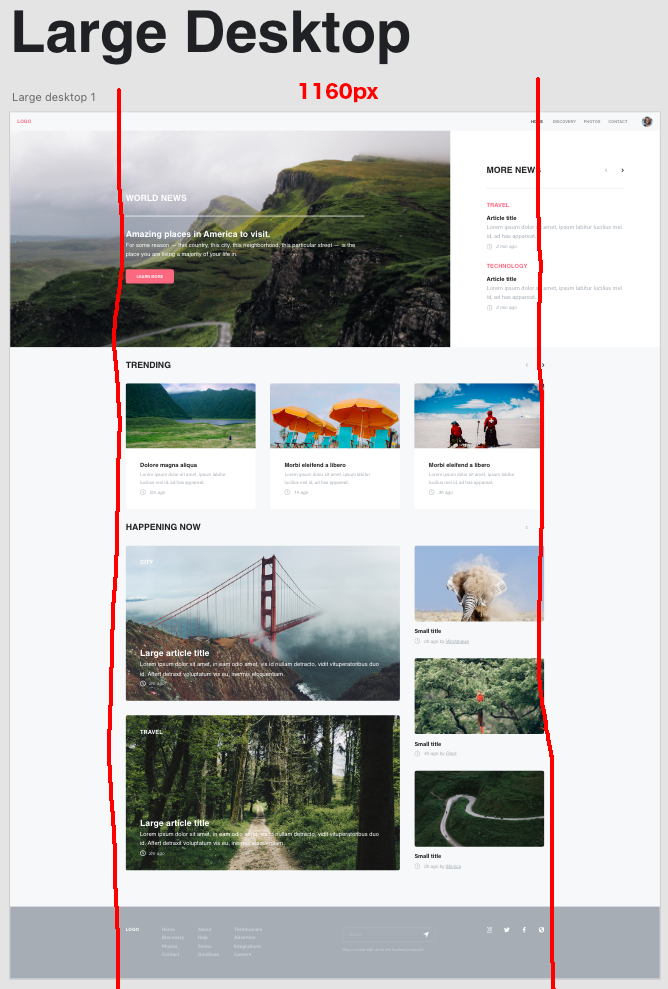
\includegraphics[width=5cm]{img/LD-fixedwidth.png}

上のMORE NEWSは「Large Desktop」「Desktop」どちらをみても、このラインからはみ出してますね。
WORLD NEWSはラインの中に入ってますね。(ちょっと厄介だなぁ...)

これらからレイアウトの構造を考えてみましょう。
\vspace{1em}

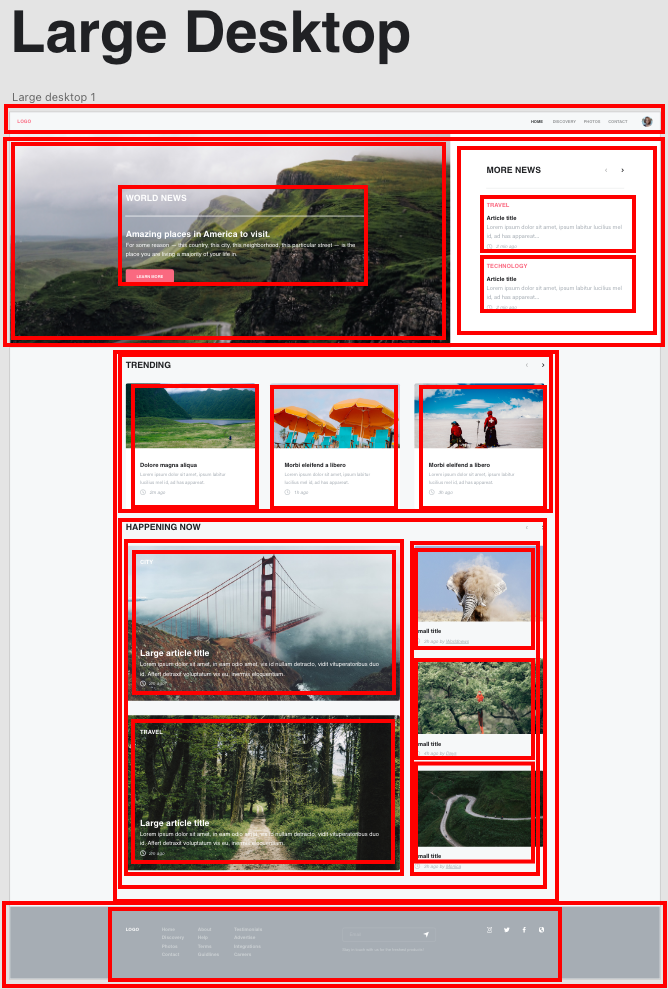
\includegraphics[width=8cm]{img/LD-block.png}

こんなふうに見えませんか?(細かいところはブロック分けできてないけど)


\section{HTML/CSSでレイアウトしていこう}
\subsection{HTMLの構造(おおまかな)}

今日のフォルダを用意して、large-desktop.htmlを準備しましょう。

タイピング練習ではないので、絵と見比べてブロックを想定して入力していきましょう。

なお、idに関してもなるべく使わない方向でコーディングしています。\footnote{https://hsmt-web.com/blog/html-id-class/}


\begin{lstlisting}[caption=HTML部分]
<!DOCTYPE html>
<html lang="en">
<head>
    <meta charset="UTF-8">
    <meta http-equiv="X-UA-Compatible" content="IE=edge">
    <meta name="viewport" content="width=device-width, initial-scale=1.0">
    <title>Let's Coding!</title>
</head>
<body>
    <div class="contents">
        <div class="menubar">
            <h1>Logo</h1>
            <nav>ナビゲーションエリア</nav>
        </div>
        <header>
            <div class="worldnews">
                <h2>WORLD NEWS</h2>
            </div>
            <div class="morenews">
                <h2>MORE NEWS</h2>
                <div class="morenews-content">
                    <div class="morenews-child">
                        <h3>Article Title</h3>
                    </div>
                    <div class="morenews-child">
                        <h3>Article Title</h3>
                    </div>
                </div>
            </div>
        </header>
        <main>
            <section class="trending">
                <h2>TRENDING</h2>
                <div class="trending-content">
                    <div class="trending-child"><h3>Trending1</h3></div>
                    <div class="trending-child"><h3>Trending2</h3></div>
                    <div class="trending-child"><h3>Trending3</h3></div>
                </div>
            </section>
            <section class="happening-now">
                <h2>HAPPENING NOW</h2>
                <div class="happening-now-content">
                    <div class="happening-now-bigchilds">
                        <div class="happening-now-bigchild"><h3>HN Big1</h3></div>
                        <div class="happening-now-bigchild"><h3>HN Big2</h3></div>
                    </div>
                    <div class="happening-now-smallchilds">
                        <div class="happening-now-smallchild"><h3>HN Small1</h3></div>
                        <div class="happening-now-smallchild"><h3>HN Small2</h3></div>
                        <div class="happening-now-smallchild"><h3>HN Small3</h3></div>
                    </div>
                </div>
            </section>
        </main>
        <footer>
            <div class="footer-content">
                Foooter Content
            </div>
        </footer>
    </div>
</body>
</html>
\end{lstlisting}

HTML5 Outlinerでどのように表示されるか確認しておきましょう。
見た目だけでなく、HTML5としてなるべく綺麗に伝わりやすく書くよう心がけましょう。

\subsection{おおまかなレイアウトをCSS Gridで指定してみよう。}
まずは、nav,header,main,footerを定義してみよう

\begin{lstlisting}[caption=おおまかな構造のCSS]
    <style>
        * {
            box-sizing: border-box;
        }
        body {
            margin: 0px;
        }
        .contents{
            display: grid;
            grid-template-columns: 1fr 1160px 1fr;
            grid-template-rows: 50px 600px 1fr 200px;
            grid-template-areas: 
                "menubar menubar menubar"
                "header header header"
                ". main ."
                "footer footer footer";

        }
        .menubar {
            grid-area: menubar;
        }
        header {
            grid-area: header;
        }
        main {
            grid-area: main;
        }
        footer {
            grid-area: footer;
        }
    </style>
\end{lstlisting}

エリアが分かりづらかったら、background-colorを設定してみても構いません。DeveloperToolsで見てみても構いません。

要素が多いとはみ出したりしていますが、エリアのレイアウトはできていることが確認できます。

\begin{itemize}
\item *のところは、幅と高さの計算方法をレイアウトしやすいようにするおまじないです。(幅や高さに境界と内側の余白を含む)
\item bodyのところは、ブラウザのデフォルトのマージンをリセットしています。
\item grid-template-areasの". main ."のピリオドは何もアサインされないことを示しています。
\end{itemize}

\subsection{.menubarのレイアウトしてみよう}
H1大きいし、ナビゲーションエリアがはみ出しているので、とりあえずfloatで左右に飛ばしましょう。

\begin{lstlisting}[caption=.menubarのレイアウト]
        h1 {
            font-size: 16px;
            float: left;
        }
        .menubar nav {
            float: right;
        }
\end{lstlisting}

\subsection{headerのレイアウトしてみよう}
これから、色とかサイズなどはXDで調べられるところは調べて設定していきます。
XDを見ると、「Large Desktop」「Desktop」ともMORE NEWSの方が幅600pxでWORLD NEWSがその残りになってくることがわかります。


\begin{lstlisting}[caption=headerのレイアウト]
        header {
            display: grid;
            grid-template-columns: 1fr 600px;
            grid-template-areas:
                "worldnews morenews"
        }
        .worldnews {
            grid-area: worldnews;
        }
        .morenews {
            grid-area: morenews;
        }
\end{lstlisting}

\subsection{.trendingのレイアウトしてみよう}
ここって、同じものが3つ並んでるから、Flexboxが使えそうだね。

\begin{lstlisting}[caption=.trendingのレイアウト]
        .trending-content{
            display:flex;
            justify-content: space-between;

        }
        .trending-child {
            width: 360px;
            height: 350px;
        }
\end{lstlisting}

\subsection{.happening-nowのレイアウトしてみよう}
ここ、Flexbox/CSS Gridどっち使ってもいけそうなので、Flexboxで書いてみます。
左右の縦は、普通に並べると縦に並ぶので特にFlexbox/CSS Grid使いません。

\begin{lstlisting}[caption=.happening-nowのレイアウト]
        .happening-now-content {
            display: flex;
            justify-content: space-between;
            align-items: flex-start;
        }
        .happening-now-bigchilds {
            width: 760px;
        }
        .happening-now-smallchilds {
            width: 360px;
        }
        .happening-now-bigchild {
            height: 430px;
            margin-bottom: 40px;
        }
        .happening-now-smallchild {
            height: 273px;
            margin-bottom: 40px;
        }
\end{lstlisting}

なんとなくのレイアウトができてきましたね。でも、画像とかないと寂しいですね。

\section{画像}
XDでは画像を選択して、Command-EとするとPNG等で書き出すことができます。

作業フォルダの中にimgフォルダを選択してその中にHeaderの画像をheader-bg.pngとして書き出してみましょう。結構XDで深く掘っていかないと(クリックしてグループ等の中に入らないと)画像まで辿りつきません。

\subsection{header背景画像, HappeningNow背景画像}

テキストP.130あたりを参考に配置してみましょう。
幅が大きくなっていいようにmax()を使って、どちらか大きい方に合わせるようにしています。

\begin{lstlisting}[caption=header画像のレイアウト]
        .worldnews {
            background-image: url(img/header-bg.png);
            background-position: center;
            background-size: max(100%,1220px);
        }
\end{lstlisting}

HAPPENING NOW, の左の2枚も同様にhappening-now-big1.png, happening-now-big2.pngとして書き出し、配置してみましょう。

HTMLのclassが上下とも同じで、これでは別々に指定ができないので、hn-big1, hnbig2をそれぞれクラスに追加しておきましょう。

\begin{lstlisting}[caption=happening-now-big画像のレイアウト]
        .happening-now-bigchilds {
            background-position: center;
        }
        .hn-big1 {
            background-image: url(img/happening-now-big1.png);
        }
        .hn-big2 {
            background-image: url(img/happening-now-big2.png);
        }
\end{lstlisting}

\subsection{Trending画像、HappeningNowSmall画像}
それぞれ記事に関する画像ですが、普通の順番だと
\begin{itemize}
\item 画像
\item 見出し
\end{itemize}
の順になってしまいます。その書き方でも良いですが、あえて今回は
\begin{itemize}
\item 見出し
\item 画像
\end{itemize}
の順にHTMLを配置し、CSS Gridで順番を変えようと思います。

とりあえず、Trending画像、HappeningNowSmall画像をtrendingX.png, happening-now-smallX.pngとして保存しましょう。
これらは、画像の元サイズで書き出すのではなく、トリミングされた状態で書き出しましょう。

\begin{lstlisting}[caption=.trending-childのHTML変更]
            <div class="trending-child">
                <h3>Trending1</h3>
                <img src="img/trending1.png">
                <p>Lorem ipsum dolor sit amet, ipsum labitur lucilius mel id, ad has appareat.</p>
                <p class="time">2m ago</p>
            </div>
\end{lstlisting}

\begin{lstlisting}[caption=.trending-childのレイアウト]
        .trending-child {
            display: grid;
            grid-template-areas: 
                "trending-child-img" "trending-child-h3" "trending-child-p" "trending-child-time";

        }
        .trending-child h3 {
            grid-area: trending-child-h3
        }
        .trending-child img {
            grid-area: trending-child-img
        }
        .trending-child p {
            grid-area: trending-child-p
        }
        .trending-child .time {
            grid-area: trending-child-time
        }
\end{lstlisting}

grid-template-areasは横に並べても問題ないです。複数列の場合は縦に並べたほうが見やすいですが、1列の時には横でも問題ないかと思います。

同様に残りの部分
\begin{itemize}
\item Trending2,3
\item HN Small1,2,3
\end{itemize}
を修正してみましょう。

多分、ここで精一杯かな...

文字などの調整やFooterは来週に回しましょう。

\section{まとめ}
多少はみ出たりしてレイアウト崩れしているところがありますが、
\begin{itemize}
\item フォントサイズ
\item マージン・パディング
\end{itemize}
等がまだ適切に設定されていないからです。

Flexbox/CSS Gridを利用するとレイアウトは非常に明快に指定することができ、
大きなレイアウトからどんどん詰めていく、という流れが今日理解してほしいところでした。








\flushright{以上}


\end{document}